\documentclass{report}
% PACKAGES
\usepackage[utf8]{inputenc}
\usepackage{mathtools} % math and figures
\usepackage{float} % make figure appear where we want with [H]
\usepackage{filecontents}
\usepackage[numbered,framed]{matlab-prettifier}
% these packages include more math symbols you might use
\usepackage{amsmath,amsfonts,amsthm,amssymb}


% PROJECT Specific Information to Fill Out
\newcommand{\LectureTitle}{Statistical Computation}
\newcommand{\LectureDate}{\today}
\newcommand{\LectureClassName}{STA663: }
\newcommand{\LatexerName}{Nancun Li, Boyang Pan}
\author{\LatexerName}


% CONFIGURATIONS to make the report look better
\usepackage{setspace}
\usepackage{Tabbing}
\usepackage{fancyhdr}
\usepackage{lastpage}
\usepackage{extramarks}
\usepackage{afterpage}
\usepackage{abstract}

% In case you need to adjust margins:
\topmargin=-0.45in
\evensidemargin=0in
\oddsidemargin=0in
\textwidth=6.5in
\textheight=9.0in
\headsep=0.25in

% Setup the header and footer
\pagestyle{fancy}
\lhead{\LatexerName}
\chead{\LectureClassName: \LectureTitle}
\rhead{\LectureDate}
\lfoot{\lastxmark}
\cfoot{}
\rfoot{Page\ \thepage\ of\ \pageref{LastPage}}
\renewcommand\headrulewidth{0.4pt}
\renewcommand\footrulewidth{0.4pt}
\usepackage{xcolor}

\title{Fast agglomerative hierarchical clustering algorithm using Locality-Sensitive Hashing}

\begin{document}
\maketitle
\newpage


\section*{Abstract}
\textcolor{red}{250 words or less. Identify 4-6 key phrases.}
 
\section*{Background} 
\textcolor{red}{State the research paper you are using. Describe the concept of the algorithm and why it is interesting and/or useful. If appropriate, describe the mathematical basis of the algorithm. Some potential topics for the background include:}\\
What problem does it address?\\
What are known and possible applications of the algorithm?\\
LSH application\\
What are its advantages and disadvantages relative to other algorithms?\\
Advantage:Faster, noise exclusion\\
Disadvantage: limits(positive integer);take much more space when C is large\\
\textcolor{red}{How will you use it in your research?}\\

Single linkage method is a fundamental algorithm in agglomerative hierarchical clustering. It connects a pair of points or clusters with the shortest distance in each step, and finally merge all individual points into one cluster. Although this algorithm is efficient, it has a large time complexity of $O(n^2)$ because it finds the shortest distance by comparing every pair of points. \\\\To address this problem, \textit{Koga}, \textit{Ishibashi} and \textit{Watanabe} proposed an approximation algorithm, the locality-sensitive hashing (LSH), which effectively find possible near points by hashing similar points into the same buckets. Therefore, we do not have to compute a whole distance matrix, but only a few of distances are needed. This algorithm is new to us, and we are intrigued by its novelty as it is the first time we have known hashing and clustering could be combined.\\\\
LSH can be quite useful when data size is large, as it has a time complexity of $O(nB)$. Here, $B$ is the maximum number of points that are hashed into the same bucket, and $B<n$. However, we also found some limits of this algorithm. First, input data should be either positive integers or negative integers. Second, it may take up a large space when a data set has a wide range of coordinate values. 

\subsection*{LSH algorithm}
LSH is a probabilistic approximation algorithm. It hashes those data points that are highly likely close into the same "bucket", so we can efficiently find the close clusters to be merged. For a $d$-dimensional data set with a maximum coordinate value $C$, LSH first transforms each observation to a $Cd$-vector. For example, a point (2,3) in a 2-dimensional space with a maximum coordinate value 5 is transformed to $$v((2,3)) = 1100011100$$,where the first 5 digits stand for 2 and the next 5 digits stand for 3, and the number of 1's correspond to the coordinate values. This transformation still contains the location information of each observation, but it uses a binary vector instead. Then, LSH apply a hash function to the Cd-vectors, randomly picking up $k$ bits from $\{1,2,...Cd\}$, extracting the values at these k locations from the vectors to hash the observations into k-vectors, and put those observations with the same hash values into a bucket. This algorithm assumes the observations with the same hash values are highly possibly close to each other, since they share partially same values. To avoid missing the observations which are close to each other but not in the same bucket, LSH generates $l$ hash functions, so the points one hash function might miss merging is likely to be merged together by another hash function.

\section*{Description of Algorithm} 
\textcolor{red}{First, explain in plain English what the algorithm does. Then describes the details of the algorithm, using mathematical equations or pseudocode as appropriate.}\\
Based on Locality-Sensitive Hashing,  Koga et al. proposed an algorithm termed LSH-link. Compared to the original algorithm, LSH-link adds a distance threshold $r$ to include the points in a bucket within this distance only and to merge several points in one phase, so fewer layers are extracted. Additionally, they proposed a noise exclusion option at the first phase, so some noise points are not merged at the beginning.

\subsection*{LSH-link algorithm}
Koga et al. adjusted LSH by setting a distance threshold $r$ to efficiently approximate the single-linkage method. This method, instead merging all the points in the same bucket together, checks if the distance between two points in the same bucket is within $r$. A pair of points that exceeds the threshold is not merged into one cluster. An advantage of this method is that it can prevent merging the points that are not supposed to be in the same cluster. Another advantage is that fewer layers are extracted by this method than single linkage method does, because several points within $r$ are merged in one step and the their distance will be all set to be $r$, but the single linkage method merges only a pair of points in one step and their distance is the true distance, which will create much more layers in a dendrogram.

\subsection*{Noise Exclusion Option}
The noise exclusion option is an algorithm to further eliminate some possible noise points in the same bucket by setting a threshold $T$. The algorithm is operated after we obtain all the buckets from $l$ hash functions and it is only operated in the first phase. It defines 3 types of points: (a) Core point: a point that has $>T$ points are within r (b) Boundary point: a point that has $<T$ points are within r, but has $\geq 1$ neighbor point(s) that are core points (c) Noise point: a point that has $<T$ points are within r, and has no neighbor point as a core point. For the noise points, we do not count them to any one of the clusters, even if they have some neighbor points that are within $r$.
\subsection*{Steps of Algorithm}
Input: maximum coordinate value $C$, number of dimensions $d$, initial number of bits picked in a hash function $k$, number of hash functions $l$, increasing rate of $r$ $A$, noise exclusion threshold $T$.\\\\
Step 1: For each point $p$, $l$ hash values $h_1(p)$, $h_2(p)$, . . . , $h_l(p)$ are computed.
In the i-th hash table, p is stored in the bucket with index hi (p). However, if
another point belonging to the same cluster as p has already been saved in the
very bucket, p is not stored in it.\\\\
Step 2: For each point p, from the set of points that enter the same bucket as p in
at least one hash table, LSH-link finds points whose distances from p are less
than r.\\\\
Step 3: The pairs of clusters, each of which corresponds to a pair of points obtained
in Step 2, are connected. If this is the first phase, the pairs of points that contains at least one noise points are not merged into a cluster.\\\\
Step 4: If the number of clusters is larger than 1 after Step 3, r is set to a new
larger value and LSH-link advances to Step 5. Otherwise, the algorithm terminates.\\\\
Step 5: LSH-link decreases k in accordance with the increase in r . It returns to
Step 1 after generating new l hash functions by using this new k value.

\section*{Performance Evaluation}
We used simulated data sets and real data sets to evaluate the performance of LSH-link algorithm. The performance is evaluated from 2 aspects.\\\\
\indent(1) Similarity. Because LSH-link is an approximation algorithm of the single-linkage clustering. We would like them to generate similar dendrograms as possible. When the dataset size is large, it is hard to recognize if their dendrograms are close, so we use CCC (Cophenetic Correlation Coefficient) and Ratio of the sum of edge lengths in the tree to evaluate their similarity.

\begin{itemize}
\item CCC (Cophenetic Correlation Coefficient): This coefficient calculates the correlation between two distance matrices. CCC is often used for measuring the similarity between two dendrograms. We denote the CCC between two distance matrices $X$ and $Y$ by $r_{X,Y}$ which is defined in the formula below. Here, let $\bar{x}$ and $\bar{y}$ be the averages of the elements of the lower triangle matrices of $X$ and $Y$ , respectively. $r_{X,Y}$ takes a value between 0 and 1. The higher the correlation grows, the larger $r_{X,Y}$ gets. In particular, when $X$ is identical to $Y$, $r_{X,Y}$ = 1. From the viewpoint of statistics, when $r_{X,Y} \leq 0.7$, X is said to have a high correlation to Y . In this paper, the correlation between two distance matrices induced from the dendrograms generateed by LSH-link and the single linkage method is investigated.
$$CCC = \frac{\sum_{i<j}(X_{ij}-\bar{x})(Y_{ij}-\bar{y})}{\sqrt{\sum_{i<j}(X_{ij}-\bar{x})^2\sum_{i<j}(Y_{ij}-\bar{y})^2}}$$
\item Ratio of the sum of edge lengths in the tree (termed "similarity ratio" below): The single linkage method produces the minimum spanning tree for the given data. Hence, we examine the number of times the sum of edge lengths in the tree generated by the LSH-link is larger than that generated by the single linkage method. The closer the ratio is to 1, the high similarity their dendrograms have.
\end{itemize}

(2) Runtime. LSH-link is created because it is faster than single-linkage clustering, we will test the time that both algorithms need to generate the dendrogram.
\subsection*{Applications to simulated data sets} 
We generated a random 1-dimensional dataset as the simulated data.  The data size is 8. The parameters we set are $$k_0 = 4, l = 10, A = 1.2, T = 11$$
\begin{table}[H]
\centering
\begin{tabular}{cccccclll}
\hline
Index & 0 & 1 & 2 & 3 & 4 & 5 & 6 & 7 \\ \hline
x-coordinate & 2 & 8 & 0 & 4 & 1 & 9 & 9 & 0 \\ \hline
\end{tabular}
\end{table}


We illustrate the result of each algorithm through the 2-D plots below. The first graph is created by the single linkage method, and the second graph is created by the LSH-link algorithm. These 2 graphs illustrated that LSH-link obtains a similar result to single linkage method. Except that the single linkage method creates a lower layer with a distance of 0, the clusters that both algorithms creates are almost the same.

\begin{figure}[H]
	\centering
	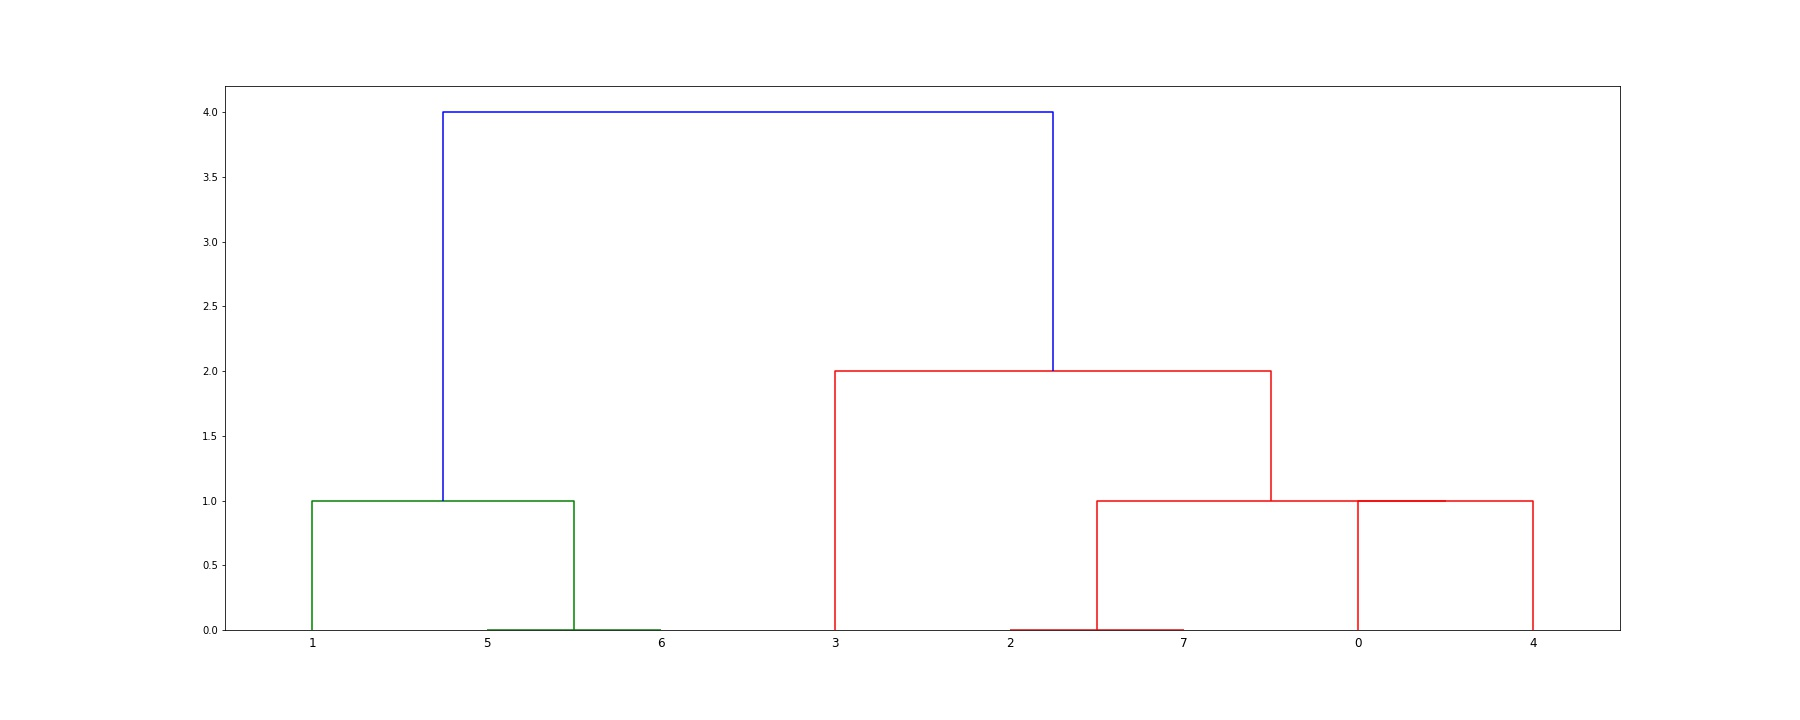
\includegraphics[width=1.0\textwidth]{figures/sim_single.jpg}
\end{figure}

\begin{figure}[H]
	\centering
	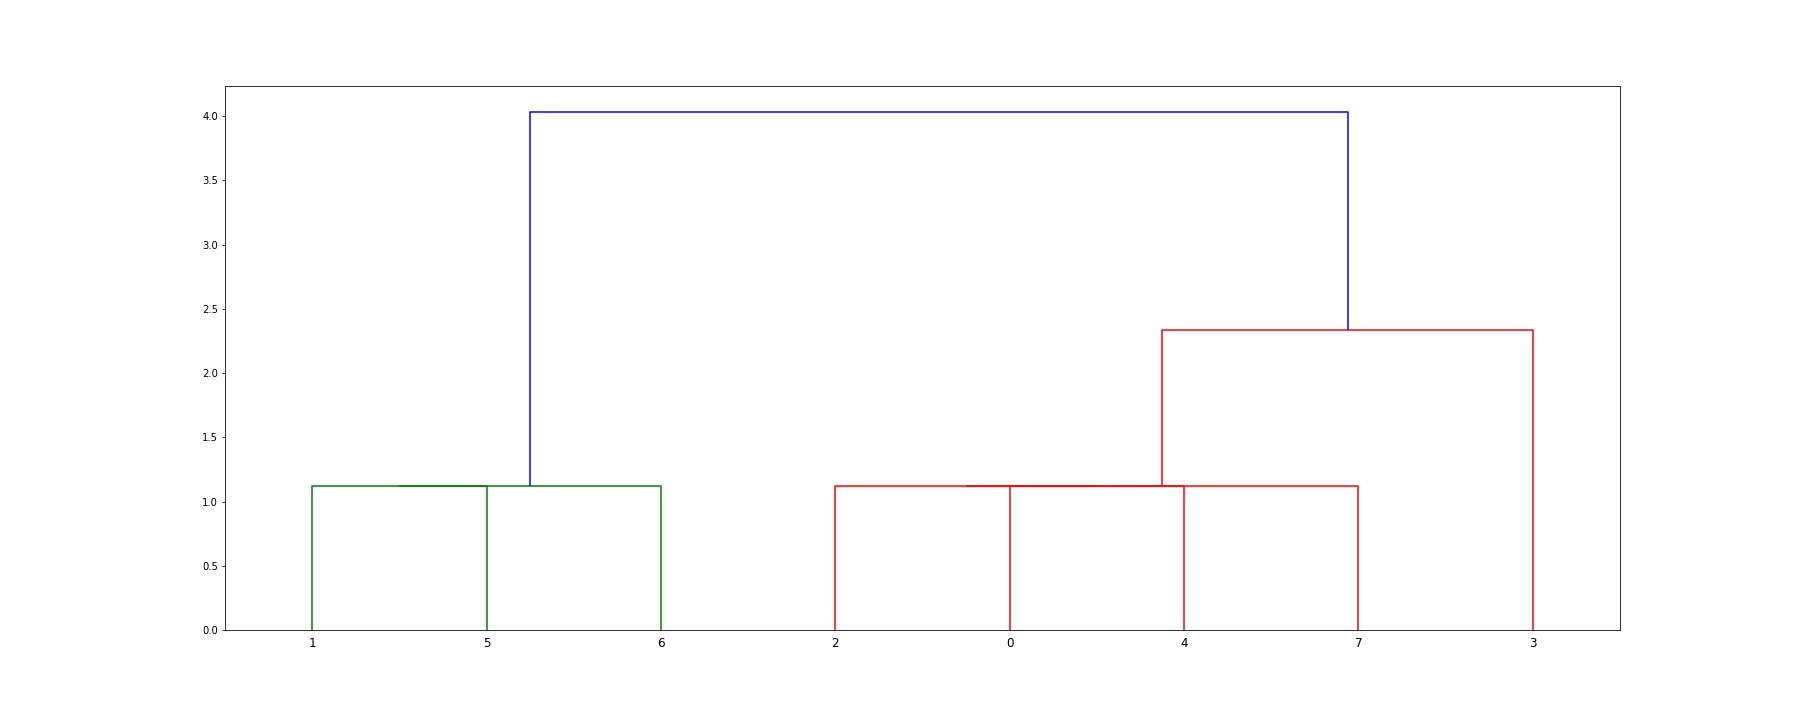
\includegraphics[width=1.0\textwidth]{figures/sim_lsh.jpg}
\end{figure}
The CCC and the similarity ratio also shows these two dendrogram are close. CCC is 0.9922, mean these two dendrograms are highly correlated. The similarity ratio of 1.33 the dendrograms are not much different.
\begin{table}[H]
\centering
\begin{tabular}{cc}
\hline
CCC & 0.9922 \\ \hline
Similarity ratio & 1.33 \\ \hline
\end{tabular}
\end{table}

\subsection*{Applications to real data sets} 
We selected the Iris Dataset from \textit{sklearn} package. This dataset has the data for 3 different types of irises. There are 150 observations with 4 parameters - Sepal Length, Sepal Width, Petal Length and Petal Width. We applied the LSH-link algorithm to this dataset trying to separate those points apart.\\\\
The parameters we set are $$k_0 = 100, l = 10, A = 2, T = 15$$
We illustrate the result of each phase through the 2-D plots below. The first graph is created by the single linkage method, and the second graph is created by the LSH-link algorithm. The dendrogram created by single-linkage algorithm has much more layers than the one created by LSH-link algorithm. However, they are not much different. Their CCC is 0.9979 and the similarity ratio is 1.28, both of which means a high similarity between the dendrograms generated.
\begin{table}[H]
\centering
\begin{tabular}{cc}
\hline
CCC & 0.9979 \\ \hline
Similarity ratio & 1.28 \\ \hline
\end{tabular}
\end{table}

\begin{figure}[H]
	\centering
	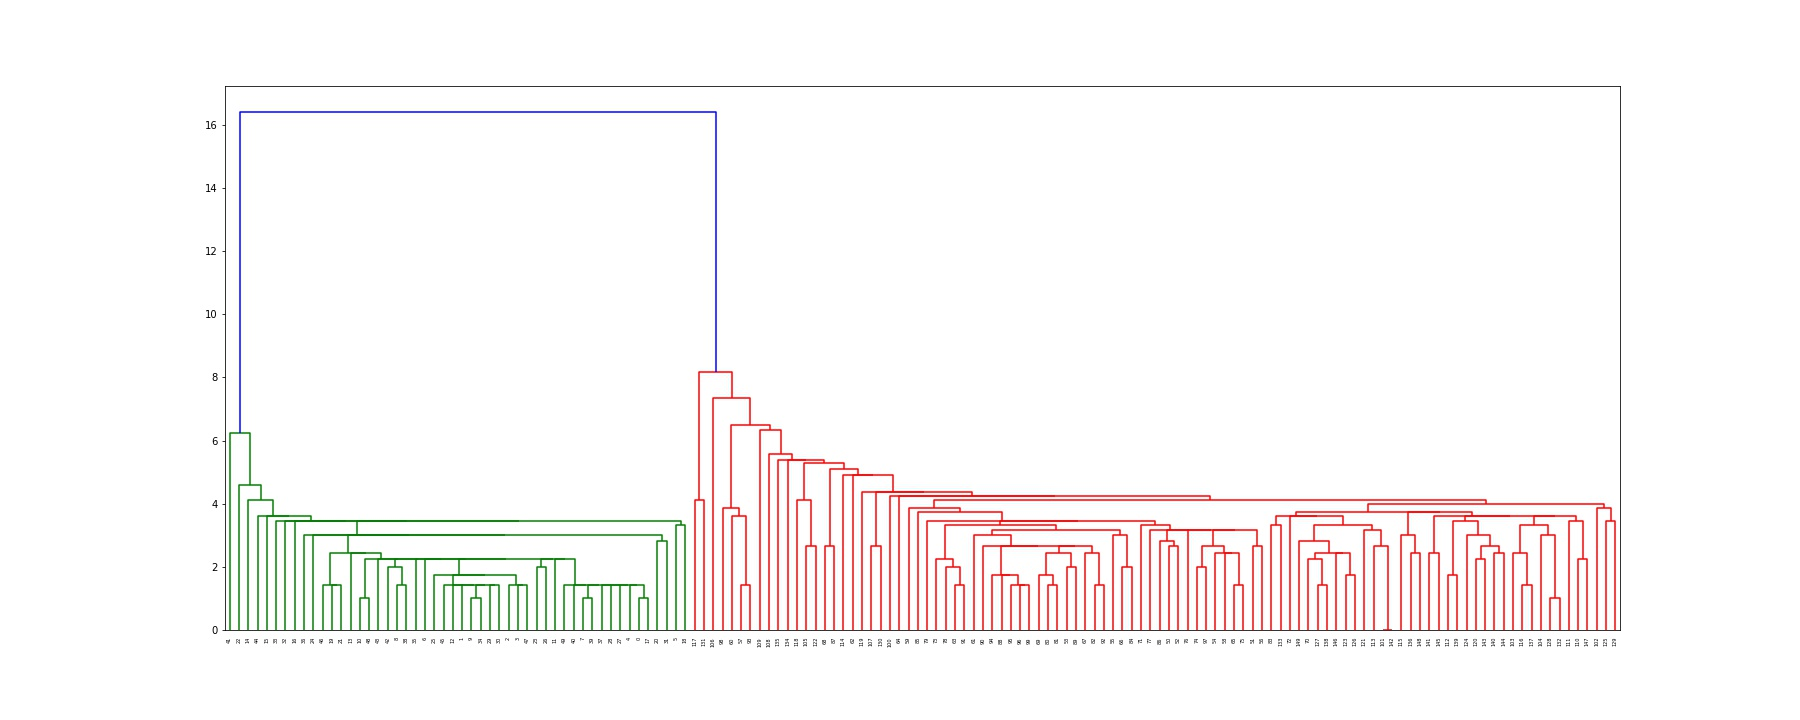
\includegraphics[width=1.0\textwidth]{figures/real_single.jpg}
\end{figure}

\begin{figure}[H]
	\centering
	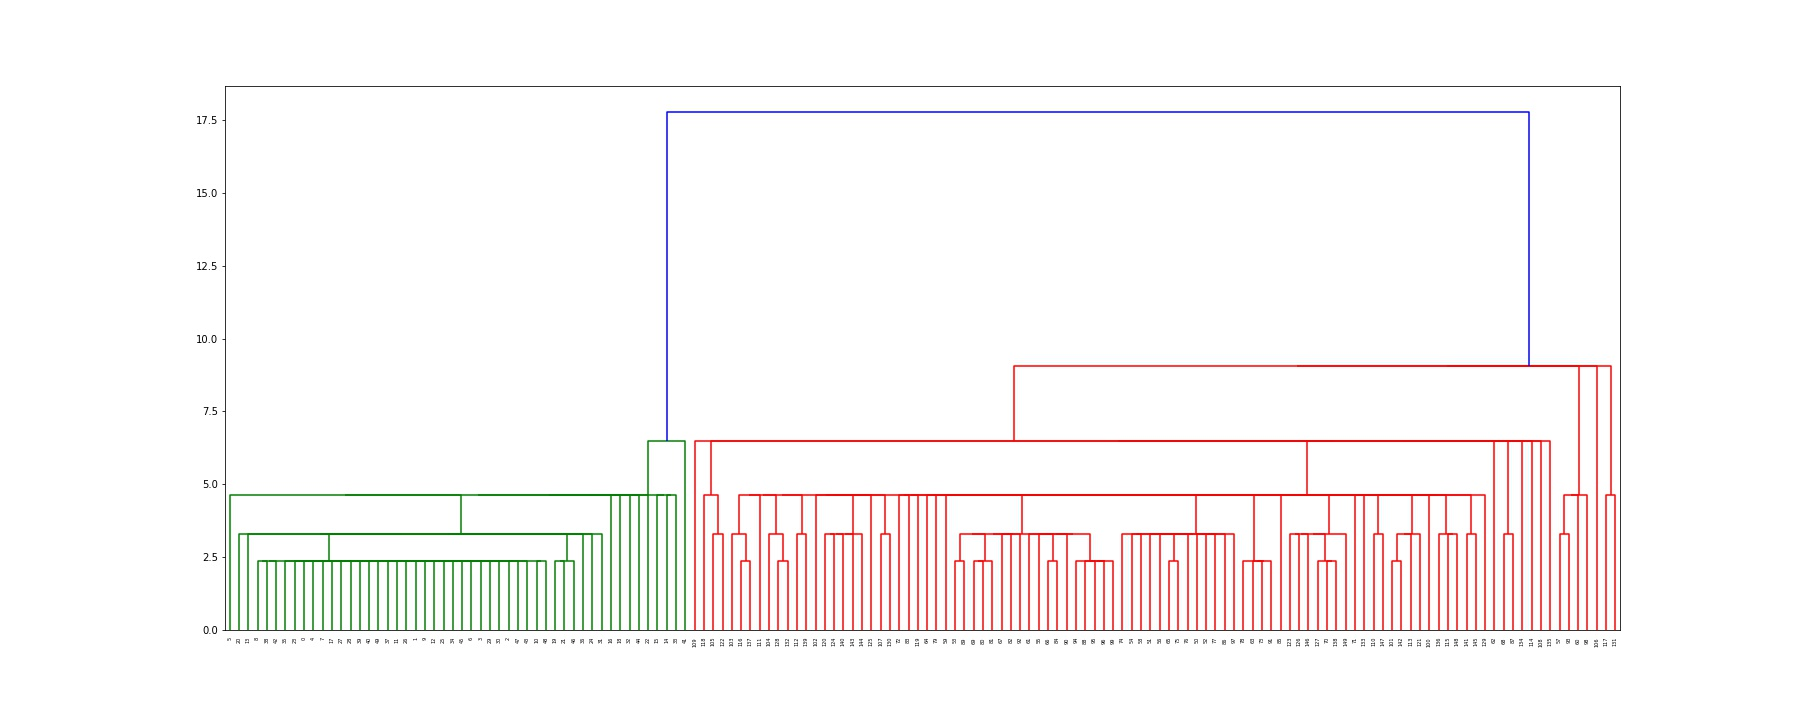
\includegraphics[width=1.0\textwidth]{figures/real_lsh.jpg}
\end{figure}

\section*{Comparative analysis with competing algorithms} 

\section*{Optimization}

\section*{Discussion/conclusion}

\section*{References/bibliography}

\end{document}





